% A useful template for typesetting beautiful homework solutions. 
% Also check out Professor Matloff's guide: 
% http://heather.cs.ucdavis.edu/~matloff/LaTeX/HowToCreate.html.
\documentclass{article}

% Packages Used
\usepackage{fancyhdr} % Required for custom headers
\usepackage{lastpage} % Required to determine the last page for the footer
\usepackage{extramarks} % Required for headers and footers
\usepackage{graphicx} % Required to insert images
\usepackage{lipsum} % Used for inserting dummy 'Lorem ipsum' text into the template
\usepackage{comment}  % Used for multi-line commenting
\usepackage{booktabs} % For better looking tables
\usepackage{array}       % for better arrays (eg matrices) in maths
\usepackage{paralist}    % very flexible & customisable lists (eg. enumerate/itemize, etc.)
\usepackage{verbatim}  % adds environment for commenting out blocks of text & for better verbatim
\usepackage{subfig}      % make it possible to include more than one captioned figure/table in a single float
\usepackage{amsthm}   % make proofs look better
\usepackage{amsfonts}
\usepackage{amsmath}
\usepackage{amssymb}
\usepackage{eufrak}      % for fraktur fonts
\usepackage{mathabx}  % for \divides
\usepackage{enumerate} % to get lists enumerated with letters
\usepackage{hyperref}  % to get attractive URLs
\usepackage{bussproofs} % for setting proofs
\usepackage{etoolbox}
\usepackage{enumitem}
\usepackage{tikz}
\usepackage{cases}

% For theorem enviornment
\theoremstyle{definition}
\newtheorem{definition}{Definition}
\newtheorem{theorem}{Theorem}[section]
\newtheorem{corollary}{Corollary}[theorem]
\newtheorem{lemma}{Lemma}

\newtheorem{mathrule}{Rule}
\newtheorem{case}{Case}
\newtheorem{subcase}{Case}[case]

\theoremstyle{plain}
\newtheorem{example}{Example}
\newtheorem{problem}{Problem}[section]

% For improved end of proof formatting
\patchcmd{\endproof}  % <cmd>
  {\endtrivlist}               % <search>
  {\endtrivlist\par\nobreak\vspace*{\dimexpr-\baselineskip-\parskip}\nobreak\noindent\hrulefill}% <replace>
  {}{}                            % <succes><failure>

% Margins
\topmargin=-0.45in
\evensidemargin=0in
\oddsidemargin=0in
\textwidth=6.5in
\textheight=9.0in
\headsep=0.25in 

\linespread{1.1} % Line spacing

% Set up the header and footer
\pagestyle{fancy}
\lhead{PHY 9HC Spring 2016\\ UC Davis - Emilija Pantic} % Top left header
\chead{} % Top center header
\rhead{\firstxmark Anze Wang ID: 912777492\\PHY 9HC A02} % Top right header
\lfoot{\lastxmark} % Bottom left footer
\cfoot{} % Bottom center footer
\rfoot{Page\ \thepage\ of\ \pageref{LastPage}} % Bottom right footer

\setlength\parindent{10pt} % Removes all indentation from paragraphs

% Common boolean operators.
\newcommand*\AND{\wedge}
\newcommand*\OR{\vee}
\newcommand*\NOT{\neg}
\newcommand*\IMPLIES{\implies}
\newcommand*\XOR{\mathbin{\oplus}}


\begin{document}

\begin{center} \bf \LARGE Homework 1\\
\end{center}


\begin {enumerate}[itemindent=30pt,label=\bf Exercise {\arabic*}:]

\item Q1B.7
\\
\\ Consider the sinusoidal traveling wave shown in figure below (This is a snapshot at a certain instant of time). Assume the wave travels at 1.0 m/s.
\\
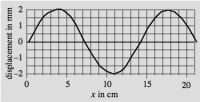
\includegraphics{q1b7}
\subitem a) What is the wave's amplitude?
\subitem \;\;\;\;The wave's amplitude is 2 mm
\subitem b) What is its wavenumber k? 
\subitem \;\;\;\;The wavnumber is $\dfrac{2\pi}{14} \approx 0.449\;\;rad/cm$
\subitem c) What is its angular frequency $\omega$
\subitem \;\;\;\;$\vert\overrightarrow{v}\vert = \dfrac{\omega}{k}$
\subitem \;\;\;\;$\omega = k\ast\vert\overrightarrow{v}\vert$
\subitem \;\;\;\;$\because \vert\overrightarrow{v}\vert = 1.0\;m/s = 100\;cm/s, k = \dfrac{2\pi}{7}$ 
\subitem \;\;\;\;$\therefore \omega = k*100 = 44.9 \;rad*s^{-1} $
\subitem d) What is its period T?
\subitem \;\;\;\;$T = \dfrac{2*\pi}{\omega}$
\subitem \;\;\;\;\;\;\;\;$= 0.14\;s^{-1}$
\subitem e) What is its frequency f? 
\subitem \;\;\;\;$f = \dfrac{\omega}{2*\pi}$
\subitem \;\;\;\;\;\;\;\;$=7.1\;Hz$
\\
\item Q1M.1
\\
\\Sinusoidal water waves are created 120km offshore by an earthquake near a small island. Observers in helicopters above the island report that the waves have an amplitude of about 2.0 m, a wavelength of 15m, and a frequency of about 0.5 Hz. How long do lifeguards on the mainland have to evacuate beaches before the waves arrive? 
\subitem $v = \lambda f$
\subitem $\because f = 0.5 Hz, \lambda = 15m$
\subitem $\therefore v = \dfrac{15}{2} m/s$
\subitem $t = \dfrac{L}{v}=\dfrac{120*10^{3}}{7.5} = 16000 s$
\\
\item Q1R.4
\\
\\ We need not have to restrict ourselves to sinusoidal wave models for waves. Consider a pulse wave described at time t=0 by the wiggle function



 \begin{numcases}{w(0,x)}
 A(1 - \vert \dfrac{x}{L} \vert), & for $|x|<L$\\ 
 0, & for $|x|>L$ 
 \end{numcases}


where A and L are constants.\\
a) Draw a graph of this wave at t=0.\\
b) What is the wave's amplitude? \\
c) Modify the function so that it maintains the same shape but moves to the right at speed $\vert\overrightarrow{v}\vert$ as time increases.Don't introduce any new constants other than $\vert\overrightarrow{v}\vert$.\\
\subitem (a)\\
\begin{tikzpicture} [domain=-4:4, line width = 2pt]
\draw[->] (-4.5,0) -- (4.5,0) node[below]{$x$};
\draw[->] (0, -4.5) -- (0,4.5) node[above]{$y$};
\draw[color=red, domain=-4.5:-2]plot(\x,0);
\draw[color=red, domain=2:4.3]plot(\x,0);
\draw[color=red, domain=0:2]plot(\x,{3 -(3/2)*(\x)});
\draw[color=red, domain=-2:0]plot(\x,{3 + (3/2)*(\x)});
\node[right = 0.5] (a) at (0,3) {A};
\end{tikzpicture}
\subitem (b)
\subitem \;\;\;\; The amplitude is equal to A.
\subitem (c)
\subitem the new function is:
\begin{equation}
   \omega(t,x) =
   \begin{cases}
   A(1 - \vert \dfrac{x-|\overrightarrow{v}|\;t}{L} \vert) &\mbox{for $|x|-\vert \overrightarrow{v} \vert\;t < L$ }\\
   0 &\mbox{for $|x|-\vert \overrightarrow{v} \vert\;t > L$}
   \end{cases}
\end{equation}
\\
\\
\item Q2B.7\\ Suppose we have a string 1.5m long that is fixed at both ends. We adjust the string's tension so the string's fundamental frequency is 100Hz. What is frequency of the normal mode of the string's oscillation that has three antinodes?
\subitem $\because$ the wave has 3 antinodes  
\subitem $\therefore n = 3 $
\subitem $\because \dfrac{f_{3}}{f_{1}} = \dfrac{3}{1} = 3$
\subitem $\therefore f_{3} = 3\;f_{1} = 3*100 = 300\;Hz$
\\
\item  Q2M.5\\Consider an organ pipe 1.72m long that has one open and one closed end. What is the fundamental pitch of this pipe? Where are the nodes (relative to the close end) for the normal model of the air in this pipe whose frequency is 150Hz?
\subitem (a)
\subitem \;\;\;\;$\because$ the speed of the wave is $340\;m/s$
\subitem \;\;\;\;$\therefore$ the fundamental pitch is $f_{1} = \frac{v}{4*l} = \frac{340}{4*1.72}= 49.42\;Hz \approx 50\;Hz$
\subitem (b)
\subitem \;\;\;\;$n = \dfrac{f_{n}}{f_{1}} = \dfrac{150}{50} = 3$
\subitem \;\;\;\;The number of nodes is equal to $n-1 = 2$
\subitem \;\;\;\;The first node is $0m$ from the close end.
\subitem \;\;\;\;The second node is $1.04m$ from the close end.
\item Q2R.1\\A sinusoidal surface wave on a body of water that significantly deeper than half the wave's wavelength has a phase speed of $$|\overrightarrow{v}| = \sqrt{\dfrac{|\overrightarrow{g}|\lambda}{2\;\pi}}$$\\where $|\vec{g}|$ is the gravitational field strength at the earth surface $9.8m/s^2$. Note that this speed depends on wavelength, so deep water is a dispersive medium for water waves. Consider standing waves in a narrow rectangular pool that has length L and is sufficiently deep. Derive an expression (in terms of  $|\vec{g}|$, L and some integer n) for the normal mode frequencies for waves in this pool. In particular, show that these frequencies are not integer multiples of some fundamental frequency. 
\begin{align*}
	f_{n} &= n\dfrac{|\vec{v}|}{2L}\\
	\qquad \qquad &=\sqrt{n^{2}\dfrac{ |\vec{g}| \lambda}{8 \pi L^{2}}}\\
	\qquad \qquad &=\sqrt{\dfrac{n |\vec{g}| }{4 \pi L}}
\end{align*}
\subitem $\because f_{n} = \sqrt{n}f_{1}$
\subitem $\therefore $ The frequencies cannot be integer multiples of fundamental frequency
\\
\\
\\
\\
\item .\\
Starting from non-relativistic Doppler formula (that we discussed during the class) derive the formula for the case of relativistic Doppler effect using material you learned in 9HB. 
\begin{figure}[h]
\begin{center}
	\begin{tikzpicture}[scale=1.5]
    		\draw[->] (-0.3,0) -- (3.5,0) node[below] {$x$};
        \draw[->] (0,-0.3) -- (0,5.5) node[left] {$t$};
        \draw[->] (0,0) -- (2.75,5.5) node[right] {$v$};
        \draw[dashed] (0.5, 1) -- (0, 2.5);
        \draw[dashed] (1, 2) -- (0, 5);
        \node[right = 0.5] at (0.5,1) {A};
        \node[right = 0.5] at (1,2) {B};
        \node[left = 0.5] at (0,2.5) {C};
        \node[left = 0.5] at (0,5) {D};        
	\end{tikzpicture}
\end{center}
\end{figure}
\subitem $v_{s}$ is the velocity of the source; $\vec{v_{\omega}}$ is the velocity of the wave; $f_{o}$ is the frequency in the home frame; $f^{'}$ is the frequency in the source frame
\begin{align*}
	t_{C} &= \gamma t^{'} + \gamma t^{'} |\dfrac{v_{s}}{\vec{v}_{\omega}}|\\
	t_{D} &= 2 \gamma t^{'} + 2 \gamma t^{'} |\dfrac{v_{s}}{\vec{v}_{\omega}}|\\ 
	f_{o} &= \dfrac{1}{t_{D} - t_{C}}\\
	\qquad\qquad &= \dfrac{1}{\gamma t^{'} + \gamma t^{'} |\dfrac{v_{s}}{\vec{v}_{\omega}}|}\\
	\qquad\qquad &= \dfrac{\sqrt{1-v_{s}^{2}}}{1+|\dfrac{v_{s}}{\vec{v}_{w}}|} f^{'}\\
\end{align*}
\subitem if the $v_{s}$ is extremely small, the formula will become $f_{o} = \dfrac{1}{1+|\dfrac{v_{s}}{\vec{v}_{w}}|} f^{'}$, which is the non-relativistic Doppler formula.
\end{enumerate}
\end{document}
